%!TEX root = /Users/ego/Boulot/TKZ/tkz-euclide/doc_fr/TKZdoc-euclide-main.tex


\section{Définition de points par transformation; \tkzcname{tkzDefPointBy} }
Ces transformations sont au nombre de sept :

\begin{enumerate}
   \item la translation;
   \item l'homothetie;
   \item la réflexion  ou symétrie orthogonale;
   \item la symétrie centrale;
   \item la projection orthogonale;
   \item la rotation;
   \item la rotation en radian;
   \item l'inversion par rapport à un cercle
\end{enumerate}

Le choix des transformations se fait par l'intermédiaire des options. Il y a deux macros l'une pour la transformation d'un unique point \tkzcname{tkzDefPointBy} et l'autre pour la transformation d'une liste de points \tkzcname{tkzDefPointsBy}. Dans le second cas, il faut donner en argument, les noms des images ou bien encore indiquer que le nom des images est formé à partir du nom des antécédents. Par défaut l'image de $A$ est $A'$. Par exemple, on écrira~:
\begin{tkzltxexample}[]
\tkzDefPointBy[translation= from A to A'](B) le résultat est dans tkzPointResult}
\tkzDefPointsBy[translation= from A to A'](B,C){} les images sont B' et C'
\tkzDefPointsBy[translation= from A to A'](B,C){D,E} les images sont D et E
\tkzDefPointsBy[translation= from A to A'](B) l'image est B'
\end{tkzltxexample}

La variante sans (s), évite l'usage d'une boucle et d'un test et est donc plus efficace.
 
\bigskip
\begin{NewMacroBox}{tkzDefPointBy}{\oarg{local options}\parg{pt}}
\emph{L'argument est un simple point existant et son image est stockée dans \tkzname{tkzPointResult}. Soit la création est une étape intermédiaire et vous n'avez pas besoin de conserver ce point alors tant qu'aucune macro ne modifie  l'attribution de \tkzname{tkzPointResult}, vous pouvez utiliser ce nom pour faire référence au point obtenu. Si vous voulez conserver ce point alors la macro  \tkzcname{tkzGetPoint\{M\}} permet d'attribuer le nom \tkzname{M} au point.}

\medskip
\begin{tabular}{lll}
\toprule
arguments &  définition  &   exemples               \\ 
\midrule
\TAline{pt}   {nom d'un point existant}   {$(A)$}
\bottomrule
\end{tabular}


\medskip
\begin{tabular}{lll}
options     &     & exemples                         \\ 
\midrule
\TOline{translation}{= from \#1 to \#2}{[translation=from A to B](E)}
\TOline{homothety}  {= center \#1 ratio \#2}{[homothety=center A ratio .5](E)}
\TOline{reflection} {= over \#1--\#2}{[reflection=over A--B](E)}
\TOline{symmetry }  {= center \#1}{[symmetry=center A](E)}
\TOline{projection }{= onto \#1--\#2}{[projection=onto A--B](E)}
\TOline{rotation }  {= center \#1 angle \#2}{[rotation=center O angle 30](E)}
\TOline{rotation in rad}{= center \#1 angle \#2}{rotation=center O angle pi/3} 
\TOline{inversion}{= center \#1 through \#2}{[inversion =center O through A](E)} 
\bottomrule
\end{tabular}

\medskip
\noindent\emph{ L'image est seulement définie et non tracée.}
\end{NewMacroBox} 

\newpage 
\subsection{La réflexion ou symétrie orthogonale } 

\subsubsection{Exemple de réflexion} 
\begin{center}
\begin{tkzexample}[vbox]
\begin{tikzpicture}[scale=1]
 \tkzInit[ymin=-4,ymax=6,xmin=-7,xmax=3]
 \tkzClip
 \tkzDefPoints{1.5/-1.5/C,-4.5/2/D}    
 \tkzDefPoint(-4,-2){O} 
 \tkzDefPoint(-2,-2){A}
 \foreach \i in {0,1,...,4}{%
 \pgfmathparse{0+\i * 72}
 \tkzDefPointBy[rotation=center O angle \pgfmathresult](A) \tkzGetPoint{A\i} 
 \tkzDefPointBy[reflection = over C--D](A\i) \tkzGetPoint{A\i'}}
 \tkzDrawPolygon(A0, A2, A4, A1, A3)    
 \tkzDrawPolygon(A0', A2', A4', A1', A3')
 \tkzDrawLine[add= .5 and .5](C,D)
\end{tikzpicture}
\end{tkzexample}
\end{center}
 
\newpage 
\subsection{L'homothétie}  
\subsubsection{Exemple d'homothétie et de projection}

\begin{center}
\begin{tkzexample}[vbox] 
\begin{tikzpicture}[scale=1.25] 
  \tkzInit   \tkzClip 
  \tkzDefPoint(0,1){A}   \tkzDefPoint(6,3){B}   \tkzDefPoint(3,6){C} 
  \tkzDrawLines[add= 0 and .3](A,B A,C) 
  \tkzDefLine[bisector](B,A,C)                     \tkzGetPoint{a} 
  \tkzDrawLine[add=0 and 0,color=magenta!50 ](A,a) 
  \tkzDefPointBy[homothety=center A ratio .5](a)   \tkzGetPoint{a'} 
  \tkzDefPointBy[projection = onto A--B](a')       \tkzGetPoint{k}   
  \tkzDrawSegment[style=dashed](a',k) 
  \tkzShowLine[bisector,size=2,gap=3](B,A,C) 
  \tkzDrawCircle(a',k)  
\end{tikzpicture}
\end{tkzexample}  
\end{center}


\newpage  
\subsection{La projection }  
\subsubsection{Exemple de projection}

\begin{center}
\begin{tkzexample}[vbox] 
\begin{tikzpicture}[scale=1.5]  
 \tkzInit[xmin=-3,xmax=5,ymax=4] \tkzClip[space=.5]
 \tkzDefPoint(0,0){A}
 \tkzDefPoint(0,4){B}
 \tkzDrawTriangle[pythagore](B,A) \tkzGetPoint{C}
 \tkzDefLine[bisector](B,C,A) \tkzGetPoint{c}
 \tkzInterLL(C,c)(A,B)        \tkzGetPoint{D}
 \tkzDrawSegment(C,D)
 \tkzDrawCircle(D,A)
 \tkzDefPointBy[projection=onto B--C](D) \tkzGetPoint{G}
 \tkzInterLC(C,D)(D,A) \tkzGetPoints{E}{F}
 \tkzDrawPoints(A,C,F) \tkzLabelPoints(A,C,F)
 \tkzDrawPoints(B,D,E,G)   
 \tkzLabelPoints[above right](B,D,E,G)
 \end{tikzpicture}
 \end{tkzexample} 
\end{center}


\newpage 
\subsection{La symétrie }  
\subsubsection{Exemple de symétrie}
 
 \begin{center}
\begin{tkzexample}[vbox] 
\begin{tikzpicture}[scale=2]
  \tkzDefPoint(0,0){O}
  \tkzDefPoint(2,-1){A}
  \tkzDefPoint(2,2){B}
  \tkzDefPointsBy[symmetry=center O](B,A){}
  \tkzDrawLine(A,A')
  \tkzDrawLine(B,B')
  \tkzMarkAngle[mark=s,arc=lll,size=2 cm,mkcolor=red](A,O,B) 
  \tkzLabelAngle[pos=1,circle,draw,fill=blue!10](A,O,B){$60^{\circ}$}  
\end{tikzpicture}  
\end{tkzexample}
\end{center}

\newpage  
\subsection{La rotation }  
\subsubsection{Exemple de rotation} 

 \begin{center}
\begin{tkzexample}[vbox] 
 \begin{tikzpicture}[scale=1.2,rotate=-90] 
 \tkzInit
 \tkzPoint(0,0){A} \tkzPoint(5,0){B}
 \tkzDrawSegment(A,B)
 \tkzDefPointBy[rotation= center A angle 60](B) 
 \tkzGetPoint{C} 
 \tkzDefPointBy[symmetry= center C](A) 
 \tkzGetPoint{D} 
 \tkzDrawSegment(A,tkzPointResult) 
 \tkzDrawLine(B,D)
 \tkzDrawArc[delta=10](A,B)(C) 
 \tkzDrawArc[delta=10](B,C)(A)
 \tkzDrawArc[delta=10](C,D)(D)  
 \tkzMarkRightAngle(D,B,A)  
\end{tikzpicture}  
\end{tkzexample}  
 \end{center} 

\newpage 
\subsection{La rotation en radian }  
\subsubsection{Exemple de rotation en radian} 
 
\begin{center}
\begin{tkzexample}[vbox]
\begin{tikzpicture} 
  \tkzInit\tkzGrid[sub]
  \tkzPoint[pos=left](1,5){A} 
  \tkzPoint(5,2){B}
  \tkzDrawSegment(A,B)
  \tkzDefPointBy[rotation in rad= center A angle pi/3](B)
  \tkzGetPoint{C}  
  \tkzCompass[color=red](A,C)
  \tkzCompass[color=red](B,C) 
\end{tikzpicture}
\end{tkzexample} 
\end{center}

\newpage 
\subsection{L'inversion par rapport à un cercle }
\subsubsection{Inversion de points}

\begin{center}
\begin{tkzexample}[vbox]  
\begin{tikzpicture}[scale=2]
  \tkzDefPoint(0,0){O}
  \tkzDefPoint(1,0){A}
  \tkzDrawCircle(O,A) 
  \tkzDefPoint(-1.5,-1.5){z1}
  \tkzDefPoint(0.35,0){z2} 
  \tkzDrawPoints[fill=red,color=black,size=8](O,z1,z2)   
  \tkzDefPointBy[inversion = center O through A](z1)
  \tkzGetPoint{Z1} 
  \tkzDefPointBy[inversion = center O through A](z2)
  \tkzGetPoint{Z2} 
  \tkzDrawPoints[fill=red,color=black,size=8](Z1,Z2)    
  \tkzDrawSegments(z1,Z1 z2,Z2)
  \tkzLabelPoints(O,A,z1,z2,Z1,Z2)  
\end{tikzpicture}
\end{tkzexample} 
\end{center}  

\subsubsection{Inversion de point : cercles orthogonaux} 

\begin{center}
\begin{tkzexample}[vbox]
\begin{tikzpicture}[scale=3]
  \tkzDefPoint(0,0){O}
  \tkzDefPoint(1,0){A}
  \tkzDrawCircle(O,A) 
  \tkzDefPoint(0.5,-0.25){z1}
  \tkzDefPoint(-0.5,-0.5){z2}
  \tkzDefPointBy[inversion = center O through A](z1)
  \tkzGetPoint{Z1} 
  \tkzCircumCenter(z1,z2,Z1)\tkzGetPoint{c}
  \tkzDrawCircle(c,Z1)
  \tkzDrawPoints[color=black,fill=red,size=12](O,z1,z2,Z1,O,A) 
\end{tikzpicture}
\end{tkzexample}
\end{center}


\newpage
Il existe une variante de cette macro pour la définition de multiples images

\begin{NewMacroBox}{tkzDefPointsBy}{\oarg{local options}\parg{liste de pts}\marg{liste de pts}}
\begin{tabular}{lll}
\toprule
arguments &  exemples  &                  \\ 
\midrule
\TAline{\parg{liste de pts}\marg{liste de pts}}{(A,B)\{E,F\}}{E est l'image de A et F celle de B.}   \\
\bottomrule
\end{tabular}

\medskip
\emph{Si la liste des images est vide alors le nom de l'image est le nom de l'antécédent auquel on ajoute « ' »}

\medskip
\begin{tabular}{lll}
\toprule
options     &     & exemples                         \\ 
\midrule
\TOline{translation = from \#1 to \#2}{}{[translation=from A to B](E)\{\}}
\TOline{homothety = center \#1 ratio \#2}{}{[homothety=center A ratio .5](E)\{F\}}
\TOline{reflection = over \#1--\#2}{}{[reflection=over A--B](E)\{F\}}
\TOline{symmetry = center \#1}{}{[symmetry=center A](E)\{F\}}
\TOline{projection = onto \#1--\#2}{}{[projection=onto A--B](E)\{F\}}
\TOline{rotation = center \#1 angle \#2}{}{[rotation=center  angle 30](E)\{F\}}
\TOline{rotation in rad = center \#1 angle \#2}{}{par exemple angle pi/3}
\bottomrule
\end{tabular}

\medskip
\noindent\emph{ Les points sont seulement définis et non tracés.}
\end{NewMacroBox}

\subsection{Exemple de translation}

\begin{tkzexample}[vbox,small]
\begin{tikzpicture} 
 \tkzDefPoint(0,0){A}  \tkzDefPoint(5,2){A'}
 \tkzDefPoint(3,0){B}  \tkzDefPoint(1,2){C} 
 \tkzDefPointsBy[translation= from A to A'](B,C){} 
 \tkzDrawPolygon[color=blue](A,B,C)
 \tkzDrawPolygon[color=red](A',B',C')
 \tkzDrawPoints[color=blue](A,B,C)
 \tkzDrawPoints[color=red](A',B',C') 
 \tkzLabelPoints(A,B,A',B')  \tkzLabelPoints[above](C,C')
 \tkzDrawSegments[color = gray,->,style=dashed](A,A' B,B' C,C')   
\end{tikzpicture}
\end{tkzexample}

\newpage
\subsection{Fruit of Life}
\begin{center}
\begin{tkzexample}[vbox] 
\begin{tikzpicture}[scale=.8]
 \tkzDefPoint(0,0){O}  \tkzDefPoint(1.5,0){A}
 \tkzDrawCircle(O,A)
 \foreach \i in {0,...,5}{
  \tkzDefPointBy[rotation  = center O  angle 30+60*\i](A) \tkzGetPoint{a\i}
  \tkzDefPointBy[homothety = center O  ratio 2](a\i) \tkzGetPoint{b\i}
  \tkzDefPointBy[homothety = center O  ratio 3](a\i) \tkzGetPoint{c\i}
  \tkzDefPointBy[homothety = center O  ratio 4](a\i) \tkzGetPoint{d\i}
  \tkzDrawCircle(b\i,a\i) \tkzDrawCircle(d\i,c\i)
  }
\tkzDrawPolygon[color=red!50!Gold,ultra thick](d0,d1,d2,d3,d4,d5) 
\tkzDrawPolygon[color=red!50!Gold,ultra thick](b0,b2,b4)
\tkzDrawSegments[color=red!50!Gold,ultra thick](b0,d5 b0,d0 b0,d1 %
                              b2,d1 b2,d2 b2,d3 b4,d3 b4,d4 b4,d5)
\tkzDrawPoints[color=red!50!Gold,size=20](b0,b2,b4,d0,d1,d2,d3,d4,d5)
\end{tikzpicture}
\end{tkzexample} 
\end{center}

\newpage
\subsection{Flower of Life}

\begin{center}
\begin{tkzexample}[vbox]
\begin{tikzpicture}[scale=.6]
 \tkzSetUpLine[line width=2pt,color=orange!80!black] 
 \tkzSetUpCompass[line width=2pt,color=orange!80!black]
 \tkzDefPoint(0,0){O} \tkzDefPoint(2.25,0){A}
 \tkzDrawCircle(O,A)
 \foreach \i in {0,...,5}{
  \tkzDefPointBy[rotation= center O angle 30+60*\i](A)   \tkzGetPoint{a\i}
  \tkzDefPointBy[rotation= center {a\i} angle  120](O)   \tkzGetPoint{b\i}
  \tkzDefPointBy[rotation= center {a\i} angle  180](O)   \tkzGetPoint{c\i}
  \tkzDefPointBy[rotation= center {c\i} angle  120](a\i) \tkzGetPoint{d\i}
  \tkzDefPointBy[rotation= center {c\i} angle   60](d\i) \tkzGetPoint{f\i}
  \tkzDefPointBy[rotation= center {d\i} angle   60](b\i) \tkzGetPoint{e\i} 
  \tkzDefPointBy[rotation= center {f\i} angle   60](d\i) \tkzGetPoint{g\i} 
  \tkzDefPointBy[rotation= center {d\i} angle   60](e\i) \tkzGetPoint{h\i}
  \tkzDefPointBy[rotation= center {e\i} angle  180](b\i) \tkzGetPoint{k\i}
  
  \tkzDrawCircle(a\i,O) \tkzDrawCircle(b\i,a\i)
  \tkzDrawCircle(c\i,a\i)
  \tkzDrawArc[rotate](f\i,d\i)(-120)
  \tkzDrawArc[rotate](e\i,d\i)(180)
  \tkzDrawArc[rotate](d\i,f\i)(180)
  \tkzDrawArc[rotate](g\i,f\i)(60)
  \tkzDrawArc[rotate](h\i,d\i)(60)
  \tkzDrawArc[rotate](k\i,e\i)(60) }
 \tkzClipCircle(O,f0)
\end{tikzpicture} 
\end{tkzexample}
\end{center}

\clearpage\newpage
\subsection{Sangaku cercle et carré}
Dans cet exemple, on peut voir comment utiliser un point sans le nommer

\begin{center}
\begin{tkzexample}[vbox]
\begin{tikzpicture}[scale = 1]
   \tkzInit[xmax = 8] \tkzClip
   \tkzDefPoint(0,0){B}
   \tkzDefPoint(0,8){A}
   \tkzDefSquare(A,B)
   \tkzGetPoints{C}{D}
   \tkzDrawSquare(A,B)
   \tkzClipPolygon(A,B,C,D)
   \tkzDefPoint(4,8){F}
   \tkzDefPoint(4,0){E}
   \tkzDefPoint(4,4){Q}
   \tkzFillPolygon[color = green](A,B,C,D)
   \tkzDrawCircle[fill   = orange](B,A)
   \tkzDrawCircle[fill   = purple](E,B)  
   \tkzTgtFromP(F,A)(B)
   \tkzInterLL(F,tkzFirstPointResult)(C,D)
   \tkzInterLL(A,tkzPointResult)(F,E) 
   \tkzDrawCircle[fill = yellow](tkzPointResult,Q)  
   \tkzDefPointBy[projection= onto B--A](tkzPointResult)
   \tkzDrawCircle[fill = blue!50!black](tkzPointResult,A)
\end{tikzpicture}
\end{tkzexample}
\end{center}   

\newpage
\subsection{Constructions de certaines  transformations \addbs{tkzShowTransformation}}

 \begin{NewMacroBox}{tkzShowTransformation}{\oarg{local options}\parg{pt1,pt2} ou \parg{pt1,pt2,pt3}}
\emph{Ces constructions concernent les symétries  orthogonales, les symétries centrales, les projections orthogonales et les translations. Plusieurs options permettent l'ajustement des constructions. L'idée de cette macro revient à \tkzimp{Yves Combe}}
  

\medskip 
\begin{tabular}{lll}
\toprule
options             & défaut & définition                         \\ 
\midrule
\TOline{reflection= over pt1--pt2}{reflection}{constructions d'une symétrie orthogonale} 
\TOline{symmetry=center pt}{reflection}{constructions d'une symétrie centrale} 
\TOline{projection=onto pt1--pt2}{reflection}{constructions d'une projection}
\TOline{translation=from pt1 to pt2}{reflection}{constructions d'une translation}
\TOline{K}{1}{cercle inscrit dans à un triangle }
\TOline{length}{1}{longueur d'un arc}
\TOline{ratio} {.5}{rapport entre les longueurs des arcs}
\TOline{gap}{2}{placement le point de construction}
\TOline{size}{1}{rayon d'un arc (voir bissectrice)}
 \bottomrule
\end{tabular}

\emph{Il faut ajouter bien sûr tous les styles de \TIKZ\ pour les tracés}
\end{NewMacroBox}

\subsubsection{Exemple d'utilisation de \tkzcname{tkzShowTransformation}} 

\begin{center}
\begin{tkzexample}[latex=6cm,small]
\begin{tikzpicture}[scale=.8]
  \tkzInit[xmin=-4,xmax=4,ymin=-5,ymax=5]
  \tkzGrid \tkzClip \tkzPoint(0,0){O} \tkzPoint(2,-2){A}
  \tkzDefPoint(70:4){B} \tkzDrawPoints(A,O,B)
  \tkzLabelPoints(A,O,B)
  \tkzDrawLine[add= 2 and 2](O,A)
  \tkzDefPointBy[translation=from O to A](B) 
  \tkzGetPoint{C}
  \tkzDrawPoint[color=orange](C)  \tkzLabelPoints(C)
  \tkzShowTransformation[translation=from O to A,%
             length=2](B) 
  \tkzDrawVectors[color=orange](O,A B,C)  
  \tkzDefPointBy[reflection=over O--A](B) \tkzGetPoint{E}
  \tkzDrawSegment[blue](B,E)
  \tkzDrawPoint[color=blue](E)\tkzLabelPoints(E) 
  \tkzShowTransformation[reflection=over O--A,size=2](B)   
  \tkzDefPointBy[symmetry=center O](B) \tkzGetPoint{F} 
  \tkzDrawSegment[color=green](B,F)
  \tkzDrawPoint[color=green](F)\tkzLabelPoints(F)
  \tkzShowTransformation[symmetry=center O,%
                      length=2](B) 
  \tkzDefPointBy[projection=onto O--A](C) 
  \tkzGetPoint{H}    
  \tkzDrawSegments[color=magenta](C,H)
  \tkzDrawPoint[color=magenta](H)\tkzLabelPoints(H)
  \tkzShowTransformation[projection=onto O--A,%
                         color=red,size=3,gap=-2](C)   
\end{tikzpicture}
\end{tkzexample}
\end{center}

\subsubsection{Autre exemple d'utilisation de \tkzcname{tkzShowTransformation}} 

Vous retouverez cette figure, mais sans les traits de construction
\begin{tkzexample}[vbox]  
  \begin{tikzpicture}[scale=1.25]
  % on définit les points nécessaires 
  \tkzInit[ymin=-3]
  \tkzClip[space=1]
  \tkzDefPoint(0,0){A}
  \tkzDefPoint(8,0){B}
  \tkzDefPoint(3.5,10){I}
  \tkzDefMidPoint(A,B) \tkzGetPoint{O} 
  % syntaxe (liste de points) {liste des images} si vide on met des '
  \tkzDefPointBy[projection=onto A--B](I) \tkzGetPoint{J}
  \tkzInterLC(I,A)(O,A) \tkzGetPoints{M'}{M}
  \tkzInterLC(I,B)(O,A)  \tkzGetPoints{N}{N'}    
  \tkzDrawCircle[diameter](A,B)
   % attention plusieurs segments donc (s) espace entre les objets 
   % virgule entre les points
  \tkzDrawSegments(I,A I,B A,B B,M A,N) 
  % idem (s) et espace entre les objets
  \tkzMarkRightAngles(A,M,B A,N,B)  
  \tkzDrawSegment[style=dashed,color=blue](I,J)
  % tkzShowTransformation il y a aussi tkzShowLine 
  \tkzShowTransformation[projection=onto A--B,color=red,size=3,gap=-3](I)
  % on trace les points à la fin ainsi c'est plus propre, il n'y a rien 
  % par-dessus 
  \tkzDrawPoints[color=red](M,N)
  \tkzDrawPoints[color=blue](O,A,B,I) 
  %  \tkzLabelPoints version rapide de  \tkzLabelPoint on met automatiquement
  % $O$ etc ... sinon on traite chaque point l'un après l'autre avec
  %  \tkzLabelPoint(le point){son label}
  \tkzLabelPoints(O)  \tkzLabelPoints[above right](N,I) 
  \tkzLabelPoints[below left](M,A) 
\end{tikzpicture} 
\end{tkzexample} 
\endinput